\documentclass{article}
\usepackage[utf8]{inputenc}
\usepackage[margin=1in]{geometry}
\usepackage{graphicx}
\usepackage{natbib}
\usepackage{enumitem}
\usepackage{array}
\usepackage{gensymb}
\usepackage{indentfirst}
\graphicspath{ {Images/} }
\usepackage{float}
\usepackage[table,xcdraw]{xcolor}
\usepackage{amsmath}

\title{Physics 111A Fall 2016- Lab 7\\
Op Amps III}
\author{Joshua Levy\\Lab Partner: Alex Chuang}
\date{October 30th, 2016}

\begin{document}

\maketitle

\section{Lab Write Up}
%1
\subsection{Input Errors}
    \begin{figure}[H]
        \centering
        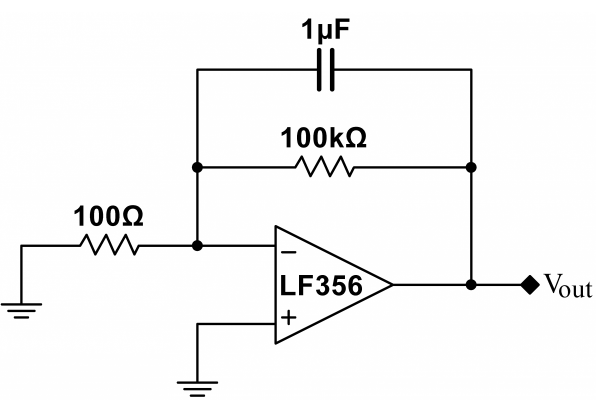
\includegraphics[scale = 0.5]{1.png}
        \caption{1000X Inverting Amplifier \cite{lab8}}
        \label{fig:my_label}
    \end{figure}
    The X1000 inverting amplifier above was built and initial and final $V_{out}$ values were found for five different op amps. The initial values were data points taken before there appeared to be voltage drift and the final values were taken after some voltage drift. Depicted in the below tables are the five op amp's $V_{out}$ values, and their corresponding input offset voltage $V_{os} = \frac{V_{out}}{1000}$:
    \begin{table}[H]
        \centering
        \caption{$V_{out}$ and $V_{os}$ values for 5 Op Amps}
        \label{my-label}
        \begin{tabular}{lllll}
        \textbf{} & \textbf{$V_{out}$} & \textbf{$V_{out}$} & \textbf{$V_{os}$} & \textbf{$V_{os}$} \\
        \textbf{Op Amp} & \textbf{Initial (mV)} & \textbf{Final (mV)} & \textbf{Initial (mV)} & \textbf{Final (mV)} \\ \hline
        1 (original) & 3710 & 3630 & 3.71 & 3.63 \\
        2 & 124 & 47 & 0.124 & 0.047 \\
        3 & -1370 & -1230 & -1.37 & -1.23 \\
        4 & 2170 & 2030 & 2.17 & 2.03 \\
        5 & 144 & 75 & 0.144 & 0.075
        \end{tabular}
        \end{table}
    Notice that the input offset voltages drifts with time closer towards 0V. We notice that this is a temperature effect because when we froze the 4th op amp, its output voltage immediately increased to 2.81V from its original initial value of 2.17V.

%2
\subsection{Balance Adjustment}
    \begin{figure}[H]
        \centering
        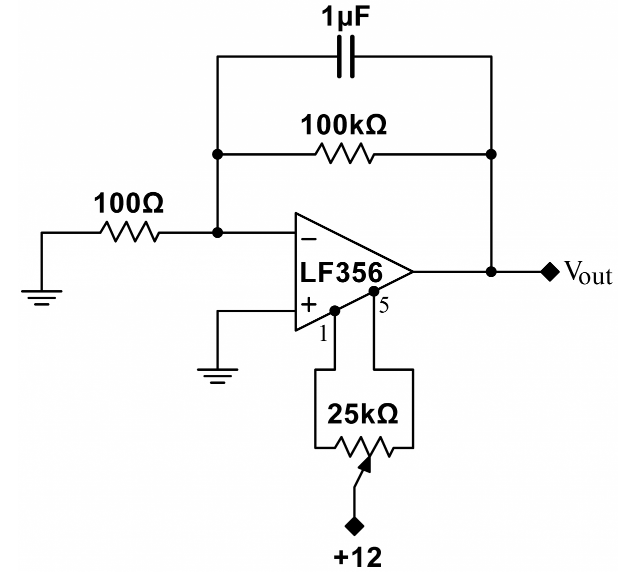
\includegraphics[scale = 0.5]{2.png}
        \caption{Balance Adjustment for Inverting Amplifier \cite{lab8}}
        \label{fig:my_label}
    \end{figure}
    A balance adjustment was added to our circuit, as depicted above. We used the original op amp from table 1 for this circuit, and adjusted the trimming potentiometer until our $V_{out}$ read to be -1.0 mV. It was really hard to get any closer to 0V than that and still have precision in our measurement. We watched its values drift over time after the adjustment. After 15 seconds, the output dropped to -50mV, and after 30 seconds, the output dropped to -99mV. As we continued to watch it over time, the output kept falling for the next few minutes. We conclude that the output drifts even after balance adjustment.

%3
\subsection{Input Bias Current}
    \begin{figure}[H]
        \centering
        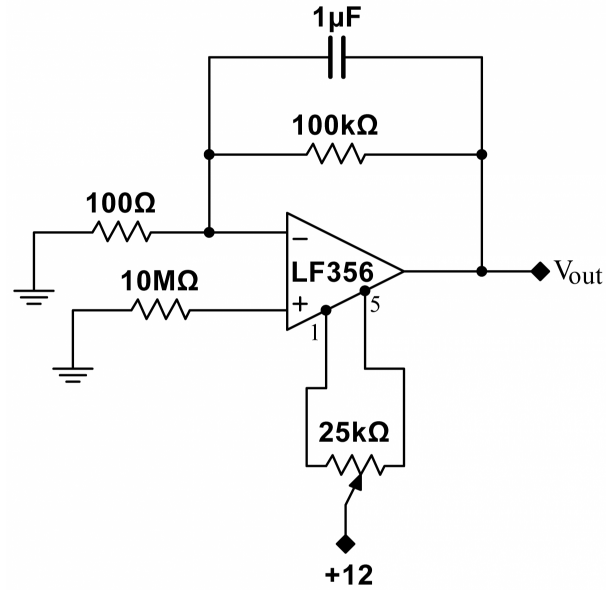
\includegraphics[scale = 0.5]{3.png}
        \caption{Using Balance Adjustment and 10M Resistor to Find Input Bias Current \cite{lab8}}
        \label{fig:my_label}
    \end{figure}
    The circuit in the above figure was built to measure the input bias current. Shorting the 10M resistor and trying to trim $V_{os}$ to 0V, the approximate value of $V_{os}$ measured to be 20 mV. With the short removed, we immediately measured $V_{os}$ to be -130 mV. We can calculate our input bias current $I_B$ by first considering $V_{out}$ and $V_-$ to form a voltage divider, of which:
    \begin{equation}
        V_- = \frac{100 V_{out}}{100k + 100}
    \end{equation}
    Then, since $V_+$ equals $V_-$, and also noting from earlier that $V_{out} = 1000*V_{os}$, we see that the current flowing through the 10M resistor is:
    \begin{equation}
        I_B = \frac{V_-}{10M} = \frac{100 V_{out}}{10M(100k + 100)} = \frac{100000 V_{os}}{10M\Omega(100k + 100)}
    \end{equation}
    This current is our input bias current, because the current flowing into $V_-$ is flowing out of $V_+$ towards ground. Taking our $V_{os}$ value above to be the $V_{os}$ measured immediately after the short was removed (with the 10M resistor) minus the $V_{os}$ measurement with the short in place, and we calculate the magnitude of the input bias current to be:
    \begin{equation}
        I_B = \frac{100000 (0.13V - (-0.02V))}{10M\Omega(100k + 100)} \approx 15 nA
    \end{equation}
    which is quite a small input bias current, which is why we usually consider the input currents into the $V_-$ and $V_+$ terminals of the op amp as negligible.

%4
\subsection{Closed Loop Op-Amp Gain Frequency Dependence}
    \begin{figure}[H]
        \centering
        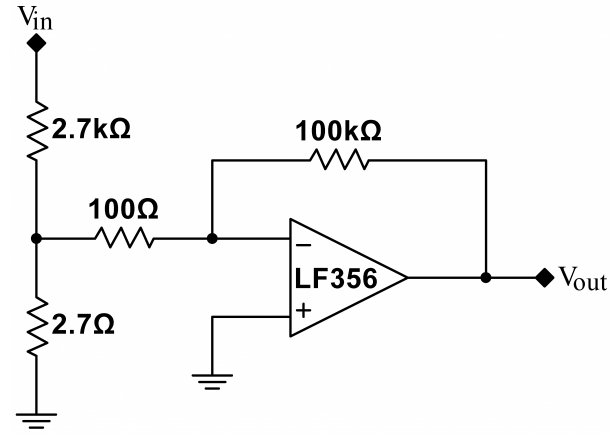
\includegraphics[scale = 0.5]{4.png}
        \caption{Inverting Amplifier Used to Find Closed Loop Op Amp Gain \cite{lab8}}
        \label{fig:my_label}
    \end{figure}
    We built the circuit above, measuring the resistance values to be $101.1\Omega, 2.76\Omega, 2.6968k, 99.05k$, in accordance with the figure's resistance values. We measured the following gain values of the inverting amplifier ($\frac{V_{out}}{V_{in}/1000}$) for the circuit:
    \begin{table}[H]
        \centering
        \caption{Closed Loop Op Amp Gain vs Frequency}
        \label{my-label}
        \begin{tabular}{lllll}
        \textbf{f (Hz)} & \textbf{$V_{in}$(mV)} & \textbf{$V_{out}$(mV)} & \textbf{Gain} & \textbf{Phase Shift ($\degree$)} \\ \hline
        10 & 960 & 1080 & 1125 & -175 \\
        100 & 960 & 1060 & 1104.166667 & -175 \\
        1000 & 960 & 1060 & 1104.166667 & -170 \\
        10000 & 960 & 540 & 562.5 & -120 \\
        100000 & 960 & 67 & 69.79166667 & -94 \\
        1000000 & 960 & 10 & 10.41666667 & -94 \\
        10000000 & 770 & 3.8 & 4.935064935 & -105
        \end{tabular}
        \end{table}
    If we plot the gain versus frequency, we wind up with the following plot:
    \begin{figure}[H]
        \centering
        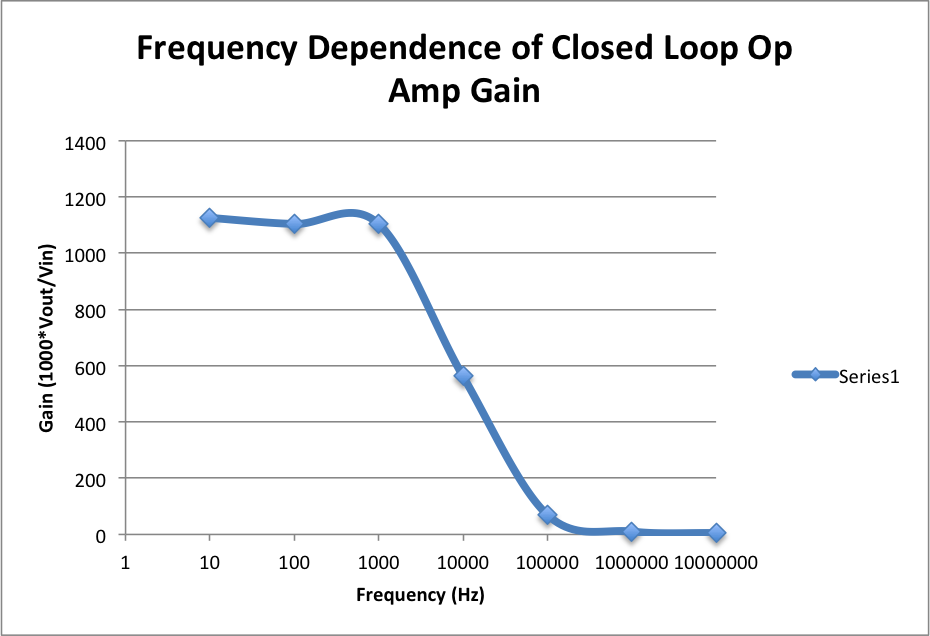
\includegraphics[scale = 0.5]{4a.png}
        \caption{Closed Loop Op Amp Gain vs Frequency Plotted}
        \label{fig:my_label}
    \end{figure}

%5
\subsection{Open Loop Gain}
    \begin{figure}[H]
        \centering
        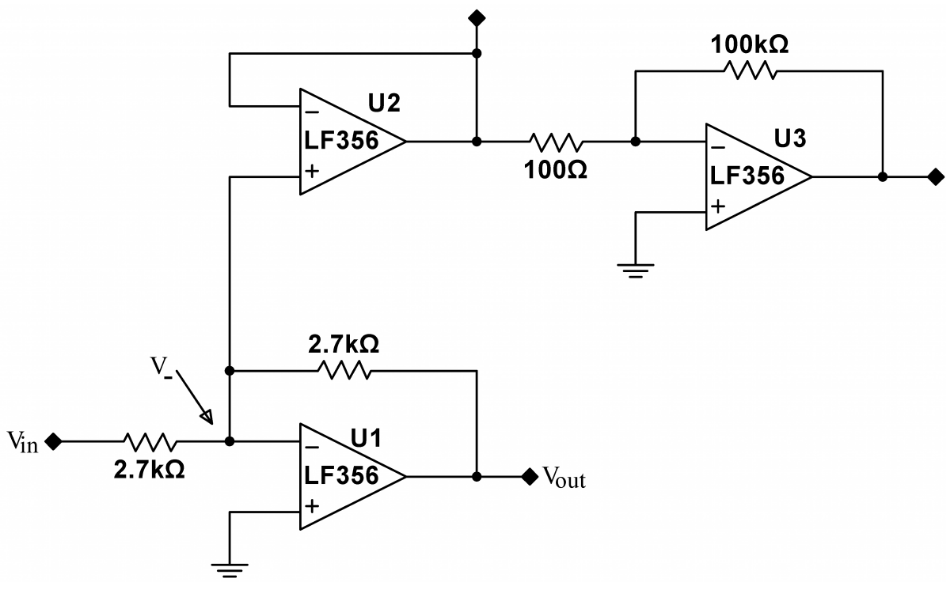
\includegraphics[scale = 0.5]{5.png}
        \caption{Circuit Used to Find Open Loop Gain \cite{lab8}}
        \label{fig:my_label}
    \end{figure}
    The open loop gain was calculated for the above circuit using the equation \cite{lab8}:
    \begin{equation}
        \displaystyle G_0 = \Bigg|\frac{V_\mathrm{out}}{V_+-V_-}\Bigg| =\Bigg|\frac{V_\mathrm{out}}{-V_-}\Bigg|
    \end{equation}
    The $V_-$ values were measured using various levels of amplifications through the use of circuit elements U2 and U3. The amplification of $V_-$ was directly modified by replacing the 100k resistor in U3 with lower valued resistors. We divided the output of U3 by the value of its feedback resistor divided by the value of its input resistor to find $V_-$. For input frequencies up to 1kHz, the 100k resistor was used in U3; from 1kHz to 10kHz, a 10k resistor was used as feedback resistor for U3, and from 10kHz to 100kHz, the U3 feedback resistor had a resistance of 1k, and for frequencies above 100kHz, a 100$\Omega$ resistor was used as a feedback resistor for U3. We measure the following values for $V_{in}$, $V_-$, and the open loop gain, $G_O$ (also measured were the  resistance values that correspond to the figure above):
    \begin{table}[H]
        \centering
        \caption{Measured Resistor Values Used in Circuit and Measured Open Loop Gain vs Frequency}
        \label{my-label}
        \begin{tabular}{lllll}
        \textbf{f (Hz)} & \textbf{$V_{in}$(mV)} & \textbf{$V_{-}$ (mV)} & \textbf{$V_{out}$(mV)} & \textbf{$G_O$} \\ \hline
        10 & 998 & 0.0158 & 1001 & 63354.43038 \\
        100 & 991.1 & 0.02875 & 1001 & 34817.3913 \\
        1000 & 987 & 0.225 & 1017 & 4520 \\
        10000 & 987.2 & 2.86 & 1040 & 363.6363636 \\
        100000 & 976 & 26.52 & 1042 & 39.29110106 \\
        1000000 & 972.8 & 214 & 1058 & 4.943925234 \\
        10000000 & 803.4 & 212.5 & 211.6 & 0.995764706 \\ \hline
        \textbf{Resistor values} & \textbf{} &  &  &  \\
        \textbf{Theoretical ($\Omega$)} & \textbf{Measured ($\Omega$)} &  &  &  \\ \cline{1-2}
        1M & 966k &  &  &  \\
        2.7k & 2.705k &  &  &  \\
        100 & 99.47 &  &  &  \\
        1k & 997.4 &  &  &  \\
        2.7k & 2.7003k &  &  &  \\
        10k & 10.07k &  &  &  \\
        100k & 99.37k &  &  & 
        \end{tabular}
        \end{table}
    We see that U2 appears to be a op amp follower, as depicted in lab 6 \cite{lab6}. We know that this is so, because when we're trying to measure $V_{-}$ above frequencies of 100kHz, we directly measure the output of U2. This is because U3 already acts like an inverting amplifier of gain -1, so you would measure the same amplitude at either U2 (the follower has a gain of approximately 1) or U3, except with an inverted signal. The function of U2 is to essentially invert the $V_-$ signal. It is an inverted follower.

%6
\subsection{Output Errors}
    \begin{figure}[H]
        \centering
        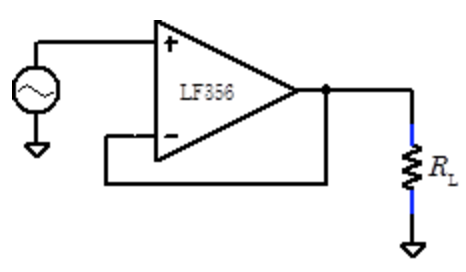
\includegraphics[scale = 0.5]{6.png}
        \caption{Follower \cite{lab8}}
        \label{fig:my_label}
    \end{figure}
    We drove the circuit above with a triangle wave. We would normally expect the circuit's output to also be a triangle wave, however, due to current limitations, we attained the following output shape for given certain load resistances:
    \begin{figure}[H]
        \centering
        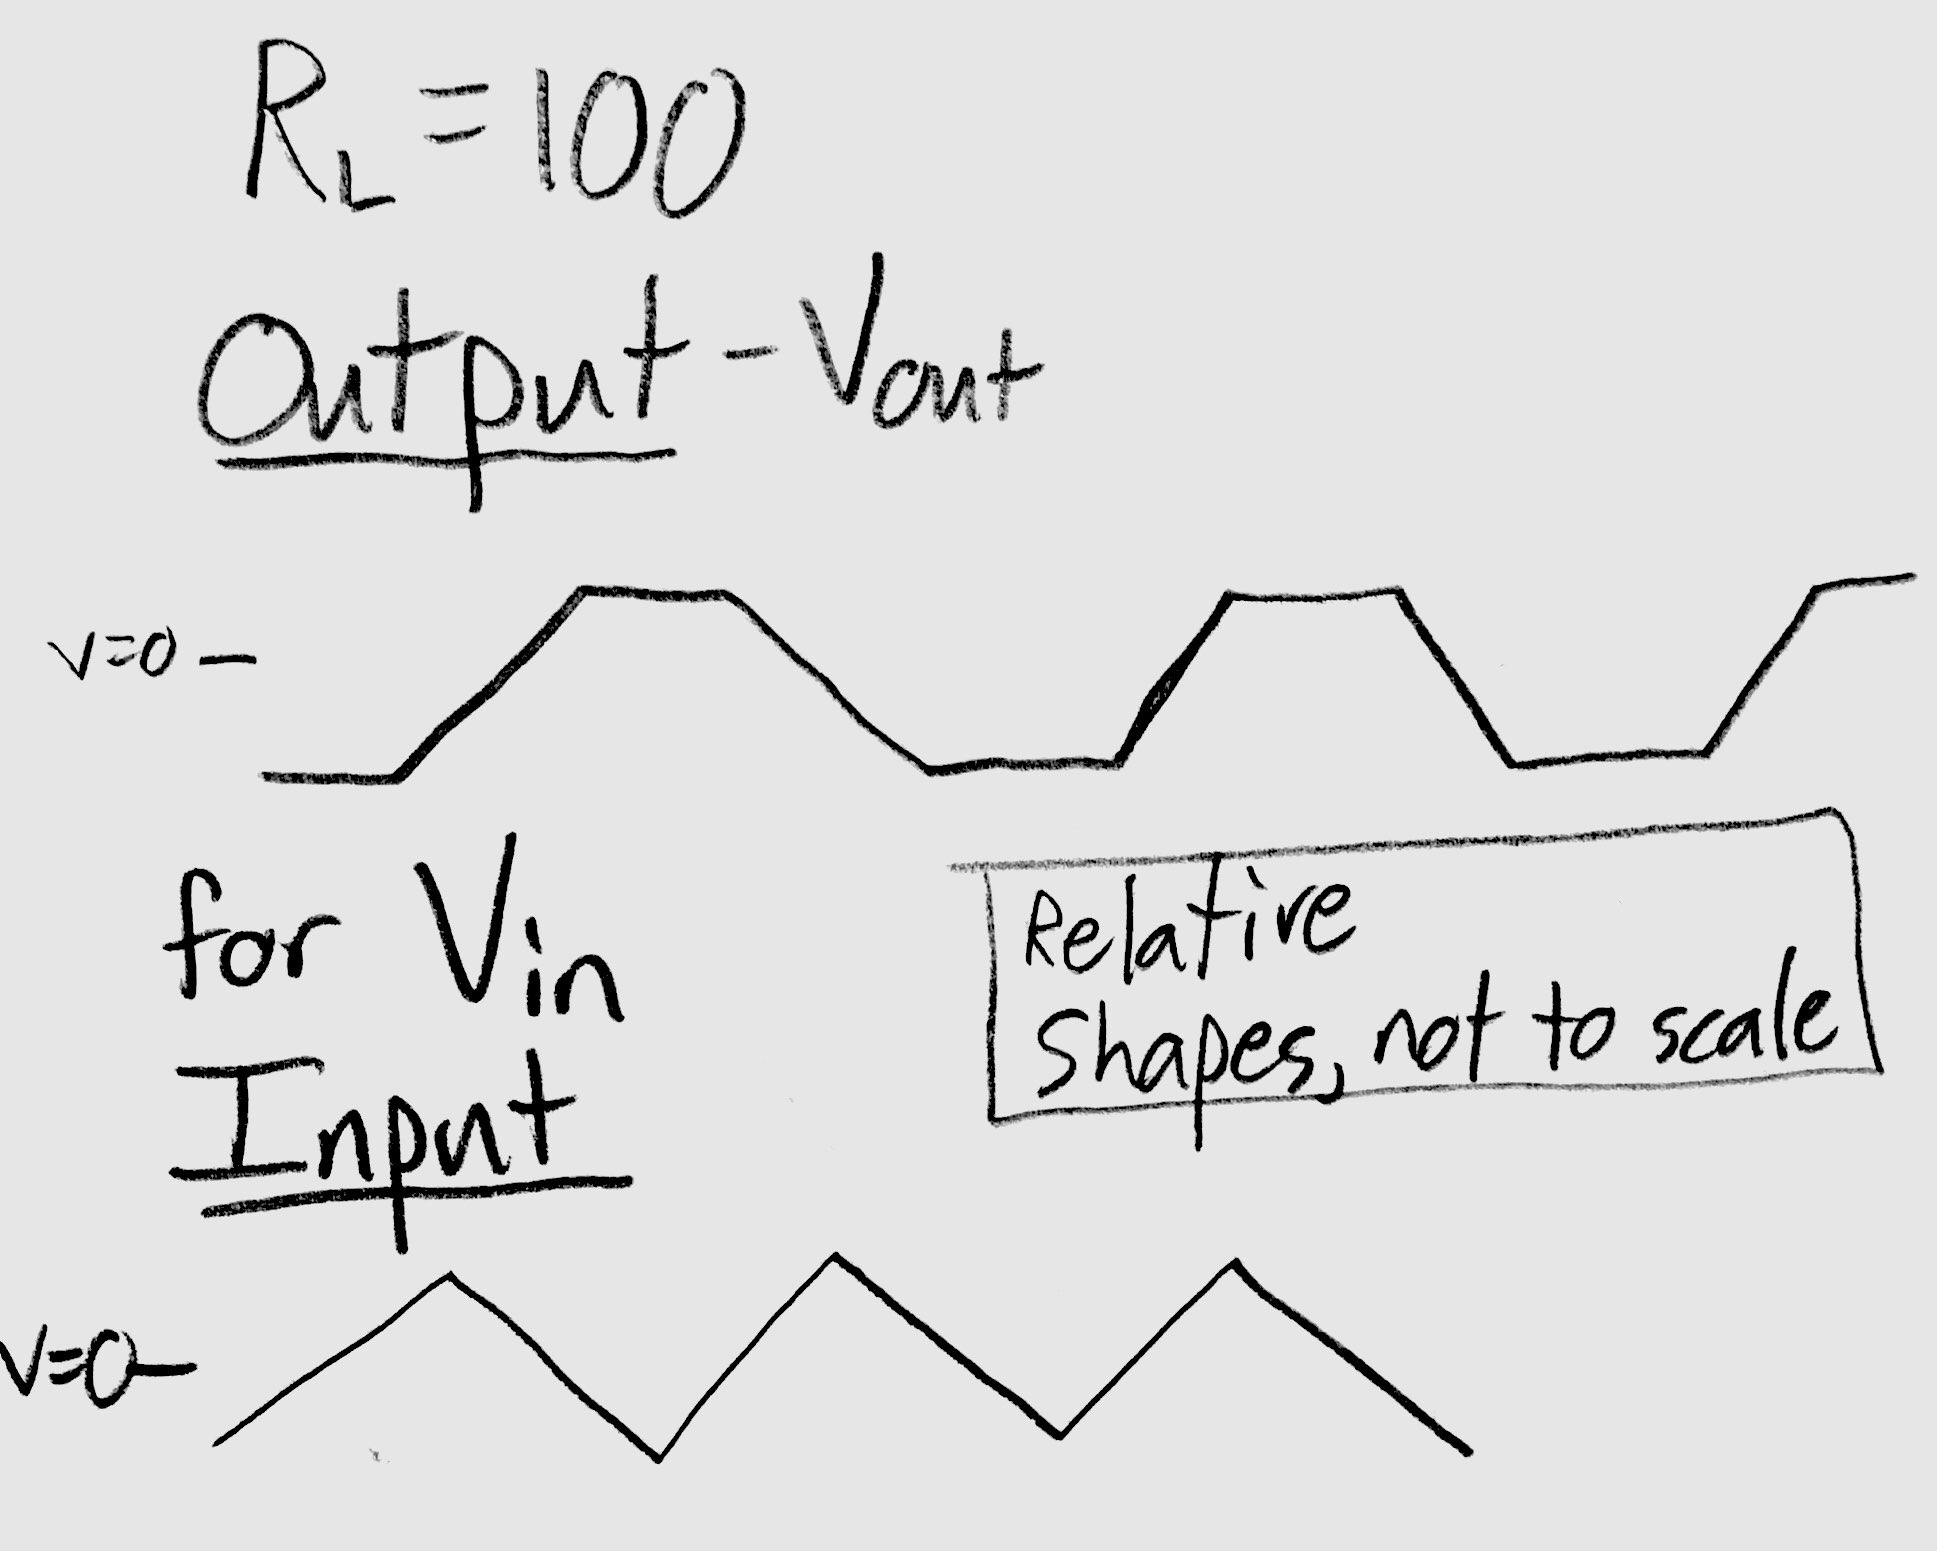
\includegraphics[scale = 0.1]{6a.JPG}
        \caption{Current Limited Output Qualitative Sketch for $V_{in}$ = 10$V_{pp}$}
        \label{fig:my_label}
    \end{figure}
    For several different load resistors, we see that the max current does not depend on $R_L$ (for the most part, with some variation) for resistance values under 200$\Omega$. At values over this, the max current drops as $R_L$ increases. We can notice this by observing some of the data points below, noting that $I_{max} = \frac{V_{max}}{R_L}$:
    \begin{table}[H]
        \centering
        \caption{Maximum output current for various load resistors}
        \label{my-label}
        \begin{tabular}{lll}
        \textbf{$R_L$($\Omega$)} & \textbf{$V_{max}$(V)} & \textbf{$I_{max}$ (A)} \\ \hline
        198 & 5 & 0.025252525 \\
        160.9 & 4.1 & 0.025481666 \\
        1000 & 5 & 0.005 \\
        99.4 & 2.7 & 0.027162978 \\
        10.1 & 0.4 & 0.03960396
        \end{tabular}
        \end{table}
    My partner and I noticed that after the $R_L$ was greater than 200$\Omega$, the output signal was triangular. We see in the above data that for all the $R_L \leq 200\Omega$, $I_{max}$ is around 0.025 A. At $R_L = 1000\Omega$, we see that the current has diminished quite a bit.

%7
\subsection{Speaker Driver}
    \begin{figure}[H]
        \centering
        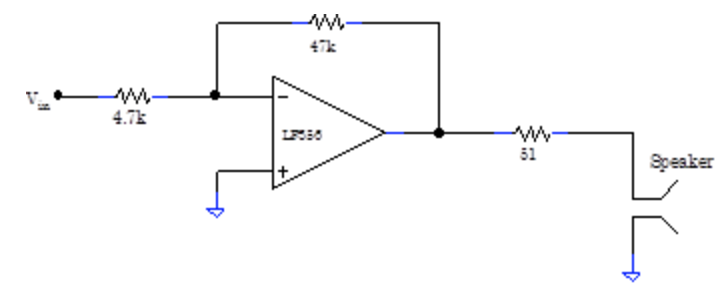
\includegraphics[scale = 0.5]{7.png}
        \caption{Preliminary Speaker Driver \cite{lab8}}
        \label{fig:my_label}
    \end{figure}
    My partner and I drove the amplifier above with sine, square and triangular waves. At first we noticed that the output sound/signal of the sine wave maintained a constant pitch for a given frequency (the sound would increase in pitch with increase in driving frequency). Then switching to the triangular wave, we again noticed a constant pitch in the output sound at that given frequency, but we could also hear some higher frequency overtones. Driving with the square wave, we noticed the output was a little bit louder and included even higher harmonics. All three wave inputs had outputs that appeared to share the same fundamental. \\\indent As we increased the amplitude of the input wave, we found that the maximum amplitude that we could drive our speaker without distortion corresponded to a input wave peak-peak amplitude of 300 mV. This is probably due to current limitations. Above the 300 mV input, the speaker probably limits the maximum/minimum voltage across it in order to limit the current passing through it so it can stay protected, thereby creating the distortion as we have seen. As we exceed this maximum amplitude, the output signal begins to distort in a way that is very similar to figure 8, albeit sine waves and square waves can be capped off if their amplitudes are too high.\\\indent The speaker is not that loud with this speaker driver, circuit, and when we switch the input to T2, we notice that the sound quality is pretty bad, that it is really hard to make out some words that people are saying, and that there is a lot of distortion in this case. I wouldn't quite say that our sound quality is acceptable at this point.

%8
\subsection{Bipolar Follower}
    \begin{figure}[H]
        \centering
        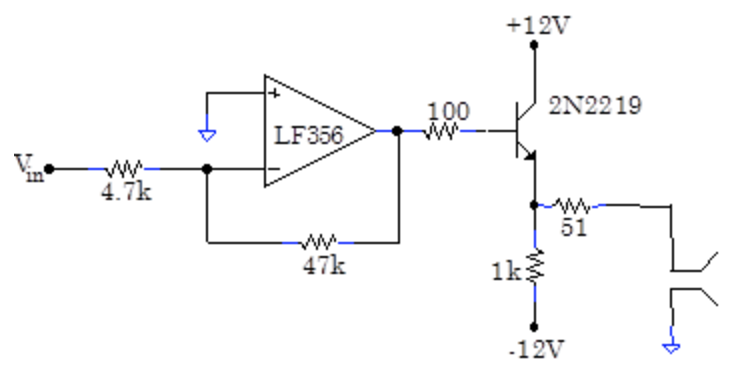
\includegraphics[scale = 0.5]{8.png}
        \caption{Bipolar Follower \cite{lab8}}
        \label{fig:my_label}
    \end{figure}
    Varying the input amplitude of sine wave inputs into the built bipolar follower as seen above, and we qualitatively attain some output wave forms as listed in the below figure for $V_{in} \in [0.01V, 1V]$.
    \begin{figure}[H]
        \centering
        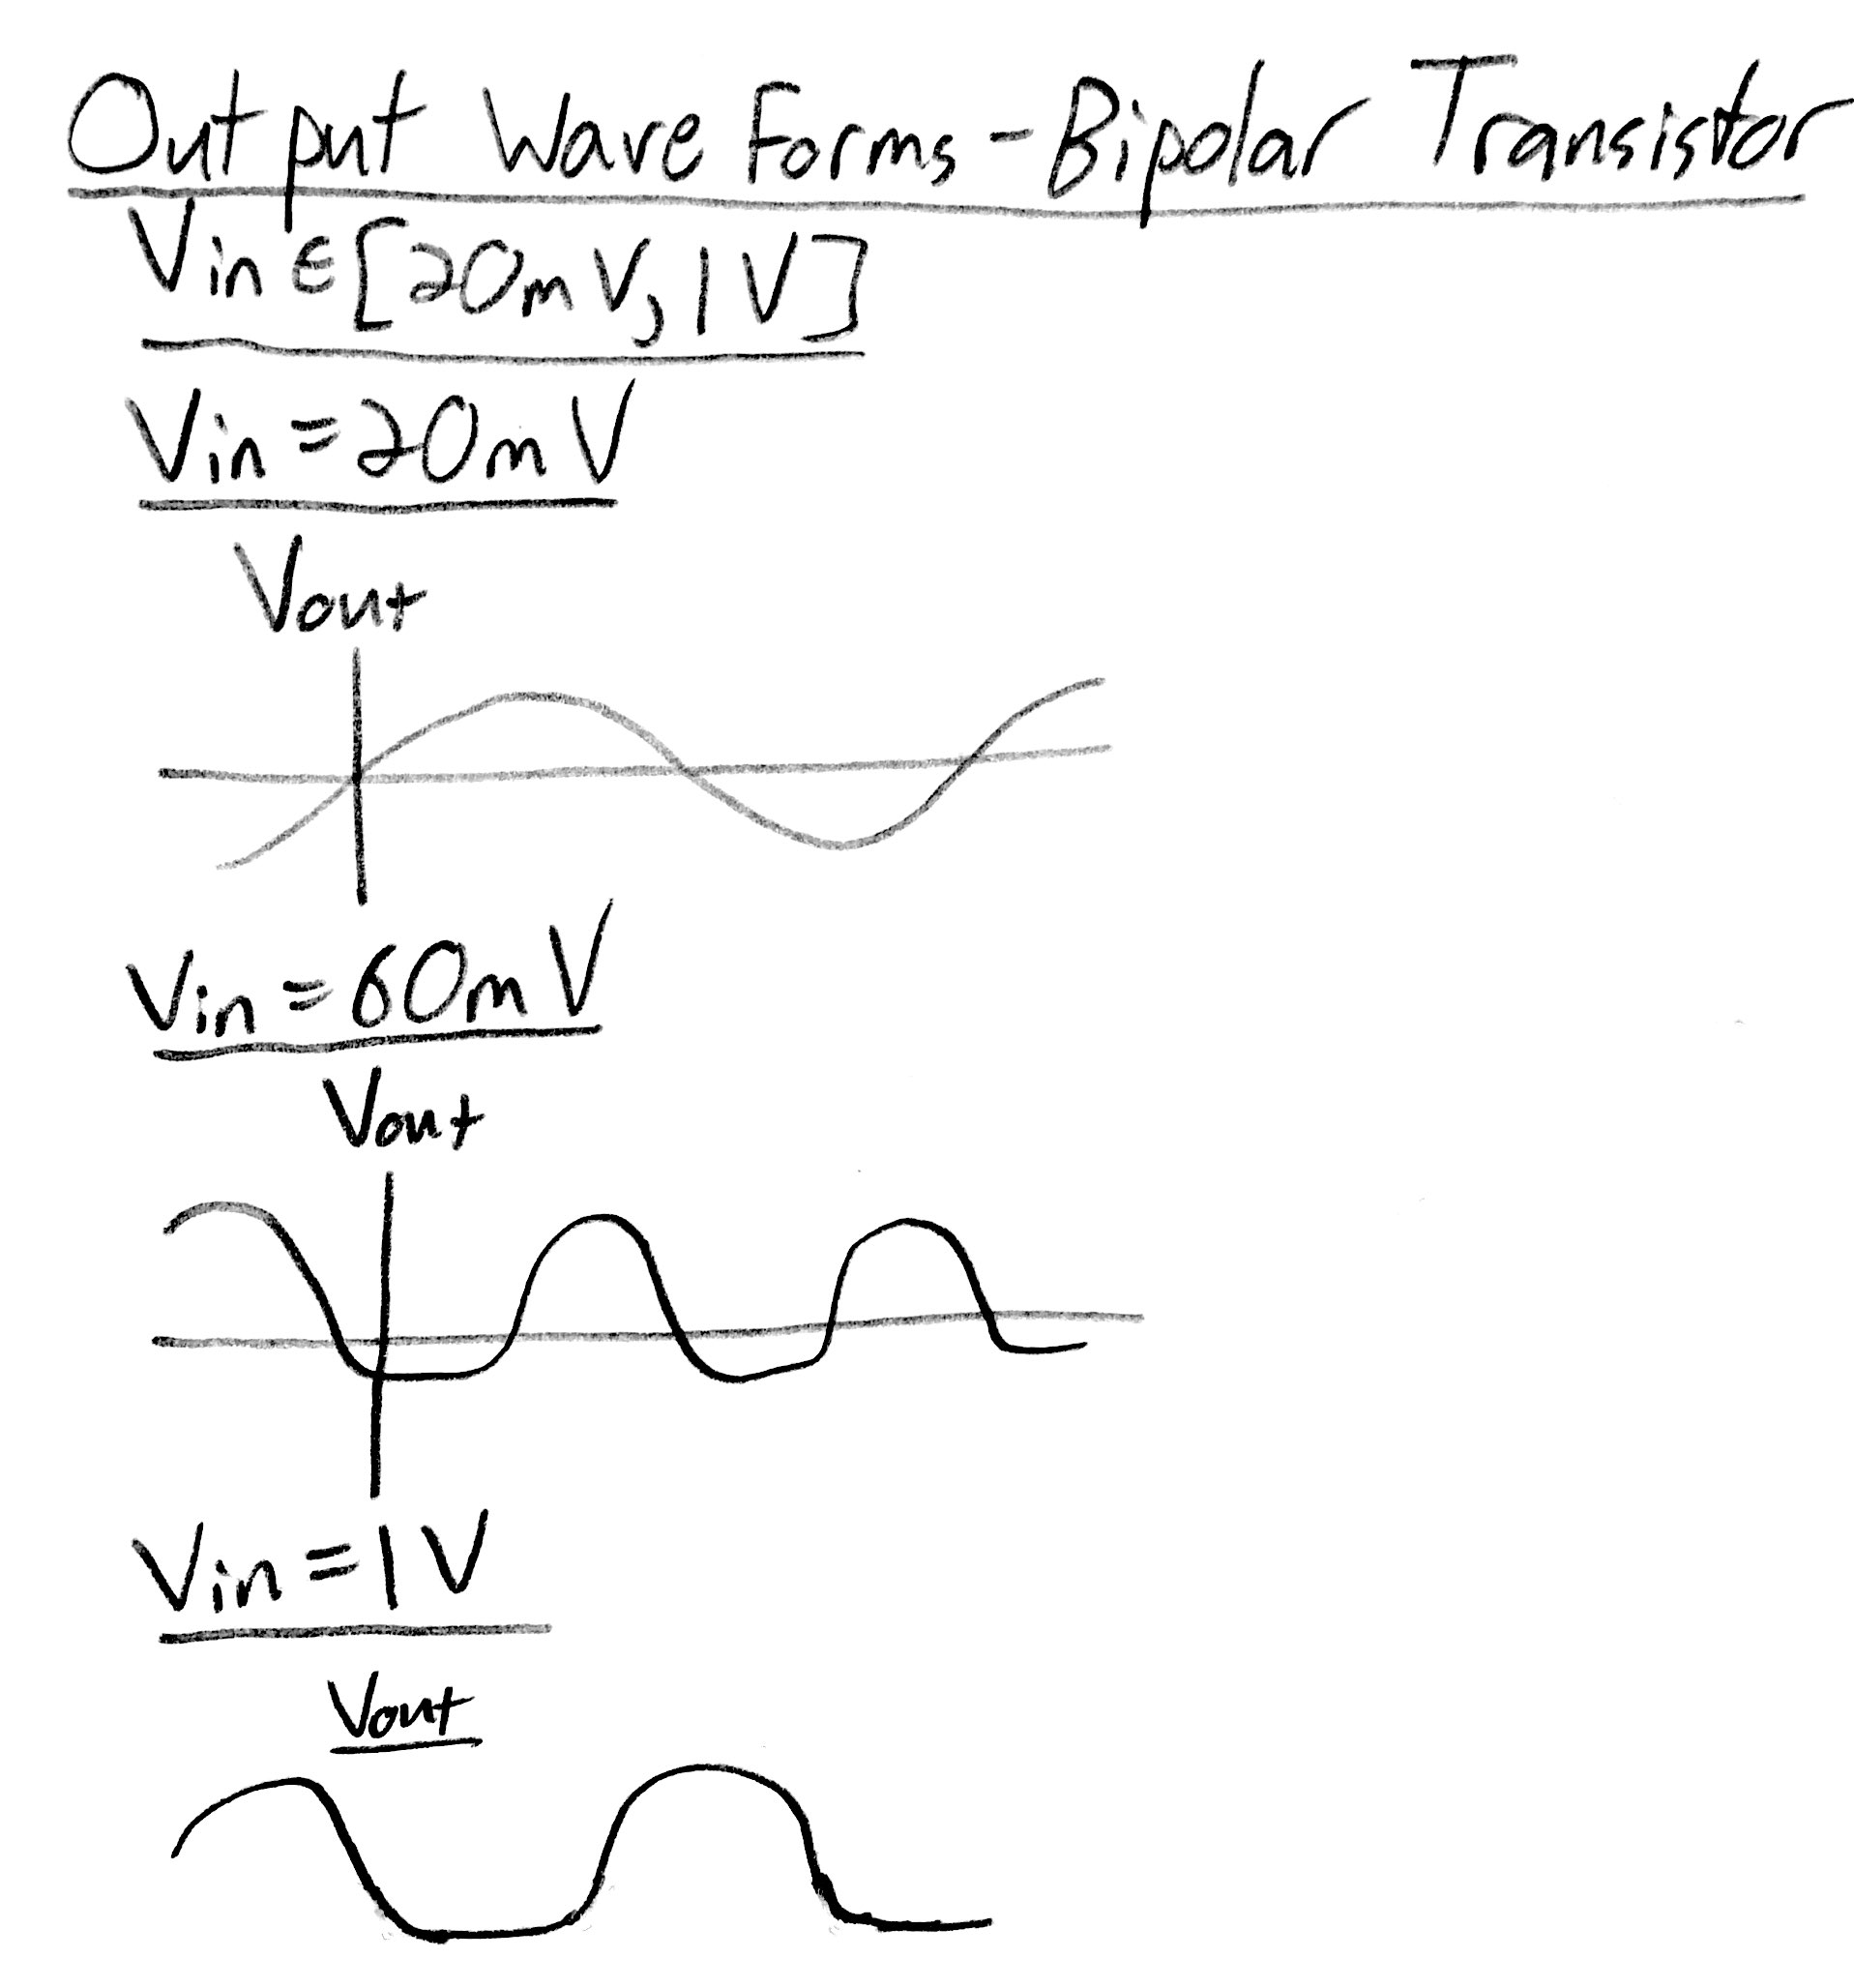
\includegraphics[scale = 0.12]{8a.jpg}
        \caption{Output Wave Forms from Bipolar Transistor, Qualitative Sketch, not to scale}
        \label{fig:my_label}
    \end{figure}
    We see that as the input amplitude increases, the output wave changes from a pure sine wave to an increasingly rectified-looking wave, where the upper half of the wave appears to look sinusoidal, but the lower half appears to be getting rectified as input amplitude increases. As you can tell by the quantitative plots, the speaker does not emit a pure sine wave at all amplitudes, and it seems that only for really low amplitudes does the speaker actually emit a pure sine wave. When driven by T2, the sound quality is a little better than the quality noticed from the previous section. It still has a long way to go.

%9
\subsection{Bipolar Follower in Feedback Loop}
    \begin{figure}[H]
        \centering
        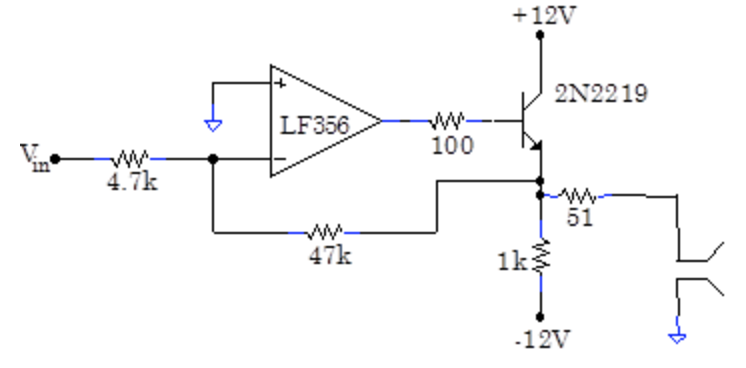
\includegraphics[scale = 0.5]{9.png}
        \caption{Bipolar Follower in Feedback Loop \cite{lab8}}
        \label{fig:my_label}
    \end{figure}
    For the bipolar follower in the feedback loop as depicted above, for input sine signals between 0.01V and 1V, the speaker emits a perfect sine wave until 300 mV, the point by which the signal starts distorting into the rectified signal as aforementioned in the previous part. This signal also becomes rectified with a vertical offset of 150mV.\\\indent The waveforms that this circuit could amplify without distortion are signals that are above this 150 mV cutoff amplitude. Anything below would have their lower portions of the signal rectified.

%10
\subsection{}
    \begin{figure}[H]
        \centering
        a)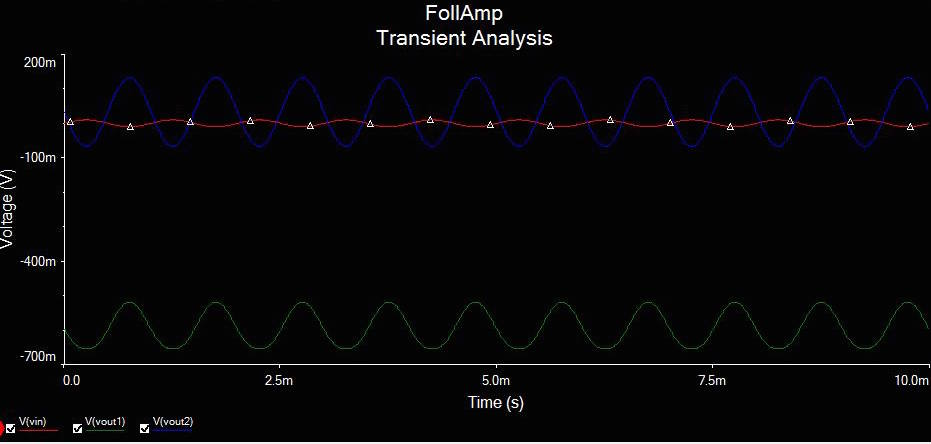
\includegraphics[scale = 0.35]{10a.jpeg}
        b)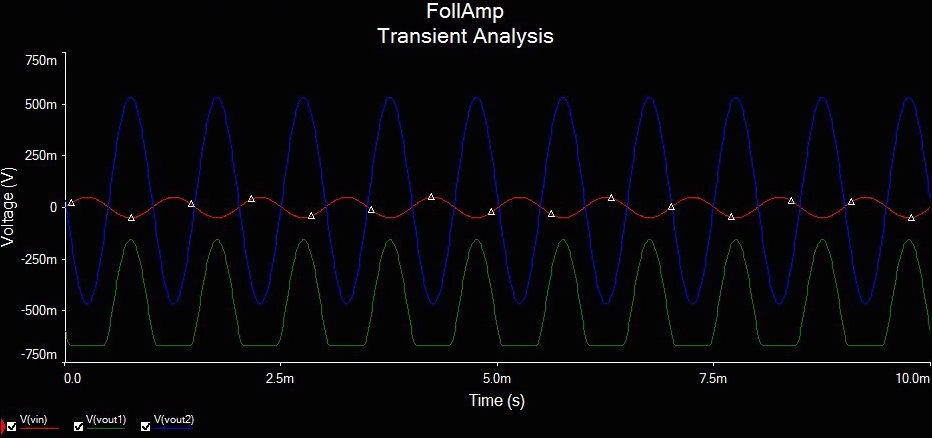
\includegraphics[scale = 0.35]{10b.jpeg}
        c)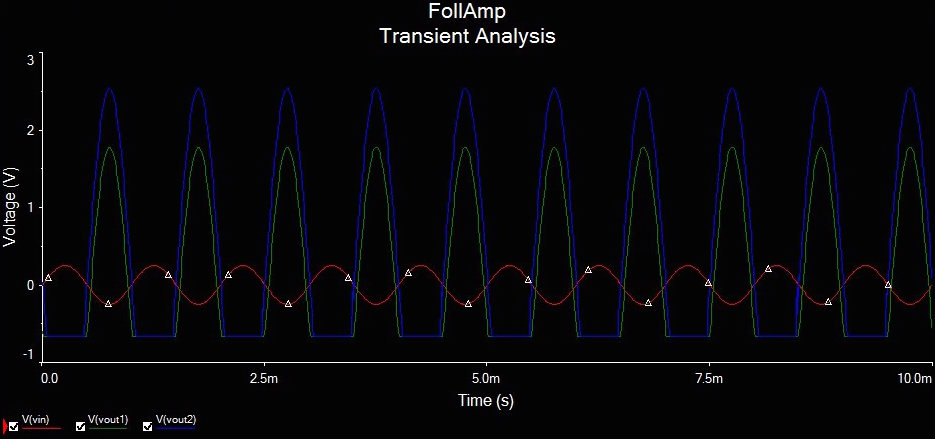
\includegraphics[scale = 0.35]{10c.jpeg}
        \caption{Multisim Transient Analyses for Circuits [1.8](green) and [1.9](blue) for input sine waves (red) of: a) 0.01$V_{pp}$, b) 0.05$V_{pp}$ and c) 0.25$V_{pp}$}
        \label{fig:my_label}
    \end{figure}
    We analyze the circuits of [1.8] and [1.9] by performing multisim transient analyses for given input amplitudes. We see that in the above figure, $V_{in}$ is the red signal, $V_{out1}$ is the green signal and describes circuit from [1.8] (figure 10), and $V_{out2}$ is the blue signal and describes circuit from [1.9] (figure 12). Figure 13a uses a 0.01$V_{pp}$ input sine wave, figure 13b uses a 0.05$V_{pp}$ input sine wave, and figure 13c uses a 0.25$V_{pp}$ input sine wave.\\\indent We see for an input 0.01$V_{pp}$ sine wave, there is a voltage offset of about -0.6V for [1.8]'s circuit (figure 11) output (figure 13a). This is because $V_{BE}$ for the bipolar transistor is 0.6V, so we expect the output to be offset by such an amount because the output of the inverting amplifier is hooked up directly into the base of the bipolar transistor.\\\indent The smaller offset (figure 13a) for [1.9]'s circuit (figure 12) output in the same input scenario is a result of the placement of the feedback connection. The output of the emitter of the transistor is fed back into $V_-$ of the op amp. We know that since $V_+$ equals 0V, that $V_-$ equals 0V, so we see that due to this negative feedback system, that $V_-$ keeps trying to establish some linearity in a the nonlinear system due to the offset in [1.8]'s circuit. It fixes any nonlinearity in the output by feeding the offset back into $V_-$ thereby bringing the offset closer to 0V ($V_E$ as well).
    \\\indent The half wave distortion for both waves at 0.25V (figure 13c) results from limitations in the bipolar transistor's polarity, that is, that it only accepts base-emitter voltages greater than 0.6V and rectifies the rest. We see here that some inversion has occurred as a result of the circuit design.
    \\\indent At 0.05V (figure 13b), we see that [1.9]'s circuit has better performance than [1.8]'s circuit (it rectifies at larger voltages) because of the feedback effect that was aforementioned. The transistor's emitter voltage is fed back into the op amp, and feeding it into $V_- \approx 0V$, which lowers the gain of the op amp and helps maintain $V_{BE}$ 0.6V levels (by reducing $V_E$) for larger frequencies than [1.8]'s circuit. The [1.8] circuit immediately feed's its output into back into it's input and the transistor base. Feeding the output of the inverting amplifier directly back into the transistor base when you're getting such amplification will cause the $V_{BE}$ to dip below the 0.6V threshold at lower input amplitudes.
    


%11
\subsection{Pushpull Driver}
    See signature page
    
%12
\subsection{Noise}
    \begin{figure}[H]
        \centering
        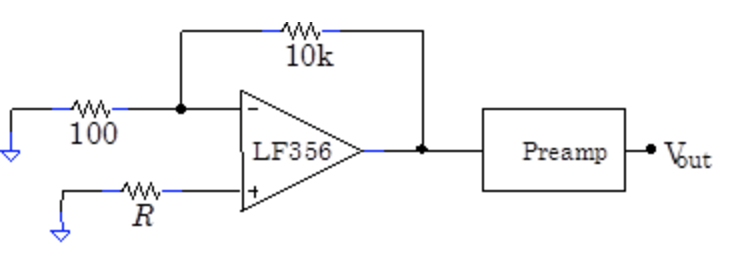
\includegraphics[scale = 0.5]{12.png}
        \caption{Preamp Johnson Noise Circuit Setup \cite{lab8}}
        \label{fig:my_label}
    \end{figure}
    We measured the Johnson noise of the preamp circuit (see the above circuit) through finding the $V_{RMS}$ of the noisy signal on both the DMM and the scope. After dividing by the 100 gain that the preamp introduced and dividing by another 100 gain that the inverting amplifier introduced (i.e. dividing total output readings on instruments by 10k): for R = 0$\Omega$, $V_{RMS}$ of the output measured to be 0.00294mV using the DMM and 0.00297mV using the oscilloscope, and for R = 1M, we measured $V_{RMS}$ to be 0.0667mV using the DMM and 0.0666mV using the oscilloscope. We compare this to our predicted Johnson Noise $V_{RMS}$, which equals \cite{Johnson}:
    \begin{equation}
        V_J = \sqrt{4kTR\Delta f}
    \end{equation}
    where k is the boltzmann constant, T is room temperature ($\approx$293K), R is the resistance in the above figure, and $\Delta$f is the bandwidth of the noise signal (equal to 100kHz-1kHz = 99kHz).\\\indent For R = 0$\Omega$, we would expect the johnson noise to be 0V. We see that our measured value is  reasonably close to that value. For R = 1M, and plugging in all the relevant factors, we would expect the Johnson Noise to be $\approx$ 0.040024 mV. This appears to agree with our measurements and is on the same order of magnitude as out measurements.



%13
\subsection{}
    We explored various types of noise using the noise generator simulation. Through our experimentation, we have come up with the following observations:
    \begin{itemize}
        \item When we generate a spectrum, we see that the amplitude histogram is still a Gaussian in shape.
        \item We changed the settings to $"1/f"$ noise, and noticed that the noise indeed sounded like distant ocean waves.
        \item Heading back to the Gaussian white noise and generate spectrum settings and setting a low pass filter to 500Hz, we notice that the output sounded like a furnace, and the reason this is so different from the $"1/f"$ noise is partially because the low pass filter did not let any higher harmonic overtones pass through, so we expect a lower pitch sound, whereas the $"1/f"$ noise has higher frequencies passing through, giving it a nice and crisp sound.
        \item The “Shot Noise” with the “Average Number of Shots per Sample” at 0.001 sounds like some static noise, like were getting discrete patterns of sound fluctuations, a very discrete albeit randomly occurring static.
        \item As we change the average number of shots per sample to 1, we see that the sound it produces starts to sound like uniform white noise of the Gaussian spectrum noise. 
        \item As we continue to increase the average number of shots per sample, at 100 the sound appears to sound like uniform white noise, at 1000 this is still uniform white noise sounding, and the noise is still soft at 10k due to the normalization of the sound. 
        \item Correspondingly, the amplitude histogram appears to become Gaussian as the randomly fluctuating noise appears to be centered around a frequency, but is randomly sampled, so a Gaussian distribution of the amplitude is relevant here. This is very consistent with the sound we are hearing, as it sounds like our Gaussian white noise, generate spectrum option.
        \item The sound volume decreases at high “Average Number of Shots per Sample” (high N) because of the normalization of the data set. If the data set was not normalized, the volume would increase as proportional to $\sqrt{N}$. However, with normalization, the normal number of fluctuations is $\frac{1}{\sqrt{N}}$, and we see that because volume is proportional to this, the volume will decrease as N increases.
        \item Changing to "Line (60Hz) Noise", and playing around with the harmonic content knob, we see that this noise is the noise that is due to the power supply. We've seen this noise before on our oscilloscopes as the noise inherent to any circuit attached to the power supply, and we have heard this sound generated before because it's the sound we hear when we tap a speaker system attached to power supply. This is the 60 Hz feedback that we're getting when we tap a speaker system. 
    \end{itemize} 

%14
\subsection{Frequency Errors}
    \begin{figure}[H]
        \centering
        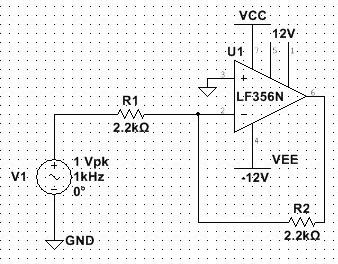
\includegraphics[scale = 0.35]{14a.jpeg}
        \caption{Direct Gn Circuit Schematic}
        \label{fig:my_label}
    \end{figure}
    Running the "DirectGn" simulation and running a transient analysis on the circuit for a given frequency, we notice that the output experiences a 180$\degree$ phase shift from the input and the circuit has a gain of -1. However, using an AC analysis, we plotted the gain and the phase shift for frequencies from 1Hz to 10GHz, and attained the following bode plot:
    \begin{figure}[H]
        \centering
        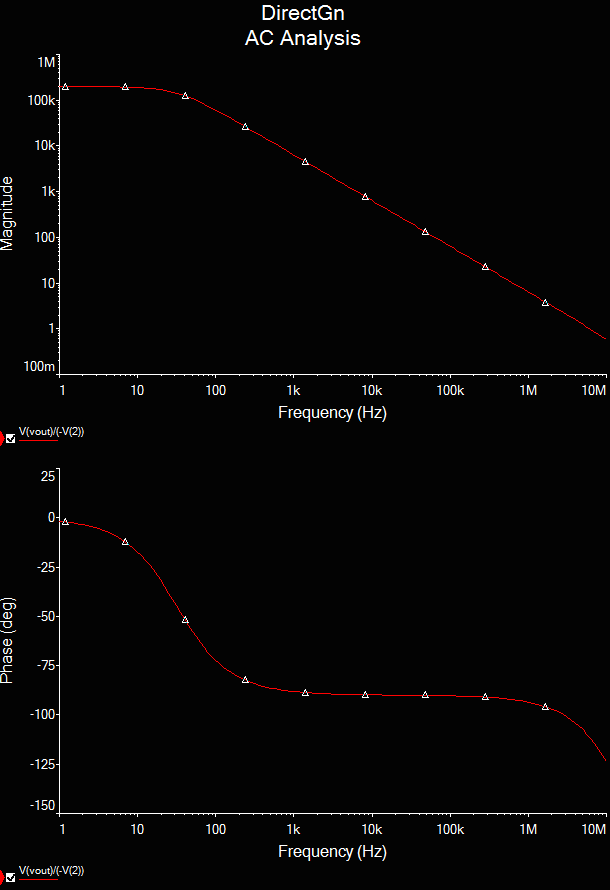
\includegraphics[scale = 0.45]{14a.png}
        \caption{Bode Plot/ AC Analysis Output of DirectGn Circuit}
        \label{fig:my_label}
    \end{figure}
    We see that there is a 0$\degree$ phase shift at really low frequencies. This value decreases to -90$\degree$, and stays there from about 1kHz to a little less than 1MHz. The shift continues to lower towards -180$\degree$ at frequencies above 1MHz. We also see that the gain continues to drop after about 50Hz at a steady rate, but does not pass below unity until frequencies larger than 1MHz.

%15
\subsection{}
    \begin{figure}[H]
        \centering
        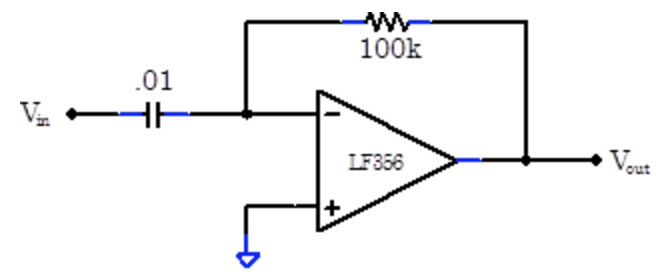
\includegraphics[scale = 0.5]{15.png}
        \caption{Differentiator \cite{lab8}}
        \label{fig:my_label}
    \end{figure}
    We constructed the differentiator above. Using op amp golden rules, we see that the rightwards current is:
    \begin{equation}
        i = C\frac{dV_{in}}{dt} = \frac{-V_{out}}{R}
    \end{equation}
    so:
    \begin{equation}
        V_{out} = -\tau \frac{dV_{in}}{dt}
    \end{equation}
    where $\tau$ is equal to RC, R being the resistance of the feedback resistor and C being the capacitance of the input capacitor. So we would expect that the circuit would differentiate its input. However, with the circuit grounded, the circuit appears to oscillate spontaneously. We looked at the scope trace of the output of the circuit, and noticed that this oscillation had a period of T = 60$\mu$s, which corresponds to a frequency of f = $\frac{1}{T}$ = 16.67kHz. Judging by the bode plot of figure 16, we notice that this oscillation frequency corresponds to an op amp phase shift of 90$\degree$. We would expect the feedback network to introduce another 90 degrees of phase shift, making the total phase shift between the input and output to be 180$\degree$. Because the circuit's phase shift is 180$\degree$ and the magnitude of the gain is greater than 1, as judged by the figure 16, we experience positive feedback effects in the circuit as $V_-$ is perfectly out of phase with the output. These feedback effects are responsible for the circuit output's oscillation.

%16
\subsection{}
    See signature page

%17
\subsection{}
    See signature page

%18
\subsection{}
    Ideally, the followers of [1.8] and [1.9] should be able to drag their outputs more negative in the case that the 1k resistor is dropped to a value closer to 51$\Omega$ because dropping this resistance value should increase the emitter current of the bipolar resistor. Because the emitter current is increased, and knowing that the base current is proportional to the emitter current, the base current increases. We know that $V_{BE}$ will increase with an increase in the base current, so the bipolar transistor should be able to accept a larger number of input signals because at lower input values, $V_{BE}$ is still above the 0.6V transistor cutoff.
    \\\indent However, the above discussion does not work in the real world because when $V_{BE}$ is much greater 0.6V, we see that the transistor heats up and either its internal resistance increases and the emitter current decreases or the bipolar transistor heats up substantially to cause the circuit component to fail/burn out.
    \begin{figure}[H]
        \centering
        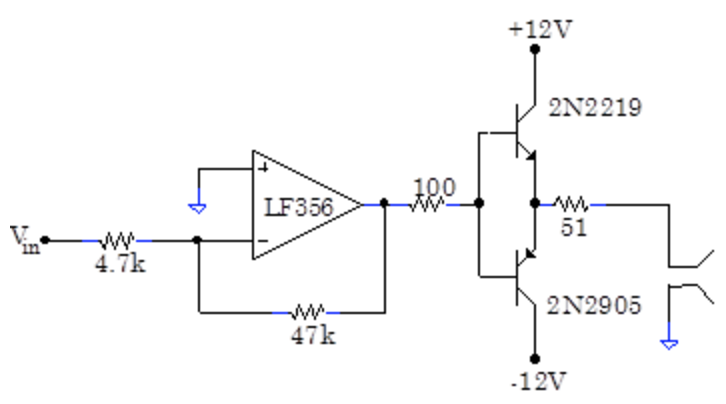
\includegraphics[scale = 0.4]{18a.png}
        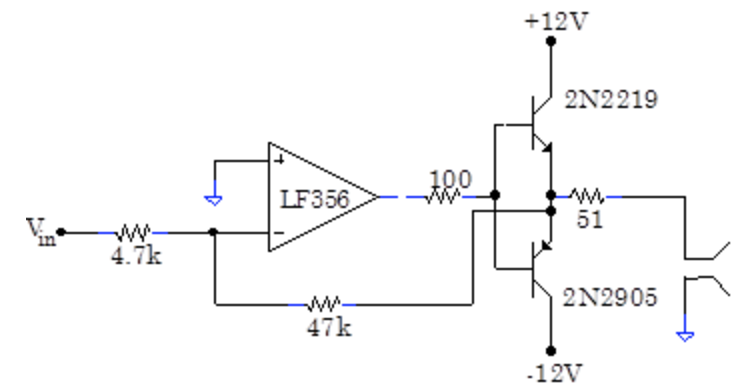
\includegraphics[scale = 0.4]{18b.png}
        \caption{Push-Pull Driver Circuit (2 different set-ups) \cite{lab8}}
        \label{fig:my_label}
    \end{figure}
    \indent The push-pull circuit (pictured above) gets around this problem because when the driving input voltage is negative, the voltage being fed into the two bipolar transistor bases is positive because of the inverting amplifier. Only the top NPN transistor will draw/pull current because $V_{BE}$ is about 0.6V, and an NPN transistor draws current at those specifications. This current is fed into our speaker system and allows the system to work in the negative input regime. If the input voltage becomes positive, the voltage at the transistor bases is negative, and only the bottom PNP transistor will draw current because $V_{BE}$ is about -0.6V, and an PNP transistor draws current at those specifications. Thus, the push-pull circuit can run the speaker with any input voltage because either the top or bottom transistor is drawing current to the speaker. This corrects the issue of trying to draw more negative voltages by correcting the bipolar followers.

%19
\subsection{}
    Calculating the gain of an inverting amplifier assuming that the open loop gain is finite, we denote $R_1$ as the input resistor to $V_-$, $R_2$ is the feedback resistor between $V_{out}$ and $V_-$, and $V_+$ is grounded ($V_+ = 0V$). We also know for finite open loop gain ($G_o$) that:
    \begin{equation}
        V_{out} = G_o*(V_+ - V_-) = -G_o*V_-
    \end{equation}
    Assuming the direct inputs to the op amp draw no current, we see that the current passing through both $R_1$ and $R_2$ are the same, and thus:
    \begin{equation}
        i = \frac{V_{in} - V_-}{R_1} = \frac{V_- - V_{out}}{R_2}
    \end{equation}
    And rearranging the equality, we get:
    \begin{equation}
        V_- = \frac{R_2*V_{in} + R_1*V_{out}}{R_1 + R_2}
    \end{equation}
    Plugging this into eq.(8), and we get:
    \begin{equation}
        V_{out} = -G_o*\frac{R_2*V_{in} + R_1*V_{out}}{R_1 + R_2}
    \end{equation}
    Rearranging this equation, we get:
    \begin{equation}
        V_{out}(\frac{R_1 + R_2+ G_o*R_1}{R_1 + R_2}) = \frac{-G_o*R_2*V_{in}}{R_1 + R_2}
    \end{equation}
    And dividing the above equality by ($\frac{R_1 + R_2+ G_o*R_1}{V_{in}*(R_1 + R_2)}$), we attain the final result for the calculated gain G, given finite open loop gain of the op amp:
    \begin{equation}
        G = \frac{-G_o*R_2}{R_1*(1+G_o)+R_2}
    \end{equation}
    Using the open-loop gain data from section [1.5] (table 3), and assuming $R_1 = 100k$ and $R_2 = 100\Omega$, and plugging into the above equation, we can predict/calculate the expected gain for the actual measured gain values in section [1.4] for various frequencies (open-loop gain is changing over various frequencies). This data is displayed below (we took the absolute values of the predicted gain and calculated relative errors between measured and expected values):
    \begin{table}[H]
        \centering
        \caption{Measured Gain vs. Predicted Gain Using Data From [1.4] and [1.5]}
        \label{my-label}
        \begin{tabular}{lllll}
        \textbf{f (Hz)} & \textbf{$G_o$} & \textbf{Measured Gain} & \textbf{Predicted Gain} & \textbf{Relative Error ($\%$)} \\ \hline
        10 & 63354.43038 & 1125 & 984.445757 & 14.2775 \\
        100 & 34817.3913 & 1104.166667 & 972.0534629 & 13.59114583 \\
        1000 & 4520 & 1104.166667 & 818.6922659 & 34.86956121 \\
        10000 & 363.6363636 & 562.5 & 266.4712544 & 111.0921875 \\
        100000 & 39.29110106 & 69.79166667 & 37.76933304 & 84.78395313 \\
        1000000 & 4.943925234 & 10.41666667 & 4.91471255 & 111.9486452 \\
        10000000 & 0.995764706 & 4.935064935 & 0.993781352 & 396.5946407
        \end{tabular}
        \end{table}
    \indent We see that the predicted gain values (generated using data from [1.5] and utilizing eq.(13)) and the measured gain values have a good level of agreement. The relative error between the measured gain and predicted gain is greater that 100$\%$ for frequencies of 10kHz, 1MHz, and 10MHz. In the case of a 10MHz input signal, the measured and predicted gain are on the same order of magnitude. Although we are getting larger than expected errors, we see that the measured and predicted gains are downwards trending (as should be expected by eq.(13)) and reasonably predictive. Therefore, we can use the data from [1.5] to reasonably predict the measured gain of [1.4] and thus conclude that the gain has some frequency dependence.

%20
\subsection{}
    See signature page





\section{Signature Page}
\begin{figure}[H]
    \centering
    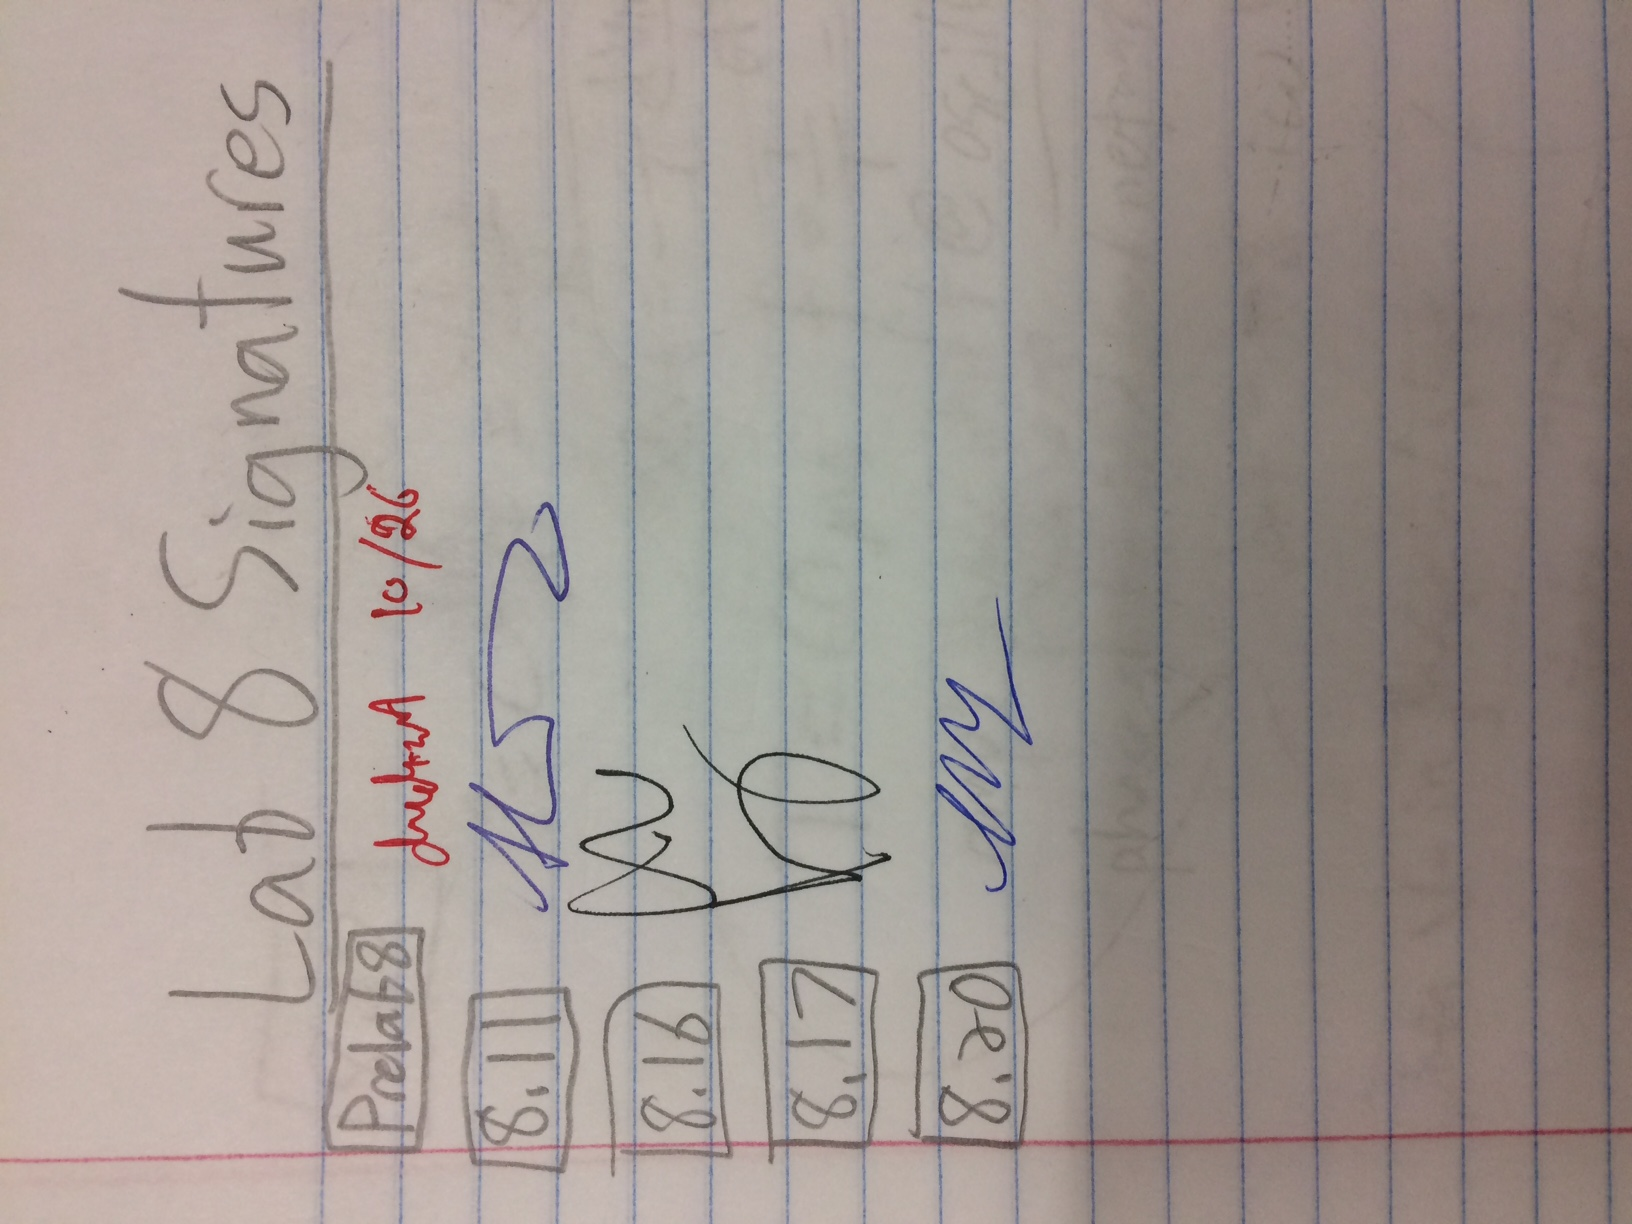
\includegraphics[scale = 0.2,angle = -90]{sig.JPG}
    \caption{Signatures}
    \label{fig:my_label}
\end{figure}



\bibliography{joshbib}{}
\bibliographystyle{plain}


\end{document}

\begin{figure}[H]
    \centering
    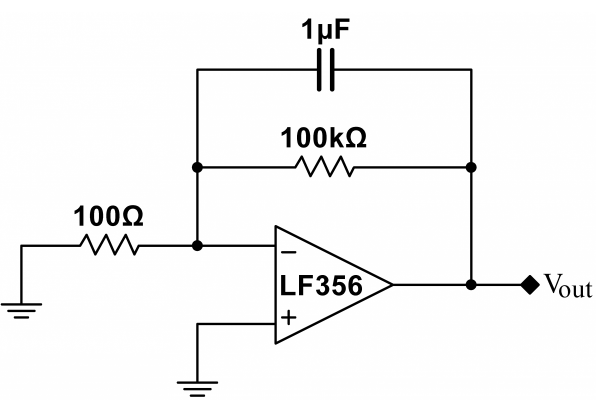
\includegraphics[scale = 0.5]{1.png}
    \caption{Caption}
    \label{fig:my_label}
\end{figure}

